\documentclass{beamer}  % This is the document class that makes presentations.
\usepackage{amsmath,amssymb,amsthm,pstricks,pst-node,pst-3d,tikz,algorithm2e}
\usetheme{JuanLesPins}
\usecolortheme{rose}

\renewcommand{\sc}[1]{\ensuremath \mathcal{#1}}
\newtheorem{question}{Question}
\newtheorem{remark}{Remark}
\newtheorem{conjecture}{Conjecture}
\newtheorem{prop}{Proposition}
\newtheorem{defn}{Definition}
\definecolor{magenta}{rgb}{0.96,0,0.722}
\definecolor{darkgreen}{rgb}{0,0.60,0}
\definecolor{cobalt}{rgb}{.239,.569,.251}
\definecolor{dpink}{rgb}{.78,.082,.522}


\title{Pattern Avoiding Permutations}
\author{Daniel Evans, Grace Hansen, \\Andrew Mortensen, Tran Khanh Tra (Fay) Nguyen}
\date{\null}

\begin{document}
\begin{frame}
\maketitle
\vspace{-.5 in}
%\begin{center}
%\includegraphics[height=37mm]{phd.jpeg}
%\end{center}
\end{frame}

%%%%%%%%%%%%%%%%%%%%%%%%%%%%%%%%
%\section{Introduction}
%%%%%%%%%%%%%%%%%%%%%%%%%%%%%%%%


%%%%%%%%%%%%%%%%%%%%%%%%%
\begin{frame}
\frametitle{Permutations and Patterns}

With $[n] = \{1,2,\ldots,n\}$ and $\mathcal{S}_n$ as the set of all possible permutations of $[n]$, we define $\pi = \pi_1\pi_2\pi_3\ldots\pi_n \in \mathcal{S}_n$ as a \textbf{permutation} of $[n]$.

Let $\sigma \in \mathcal{S}_m$ ($m \leq n$). If there exist indices $1\leq i_1 < i_2 < i_3 < \ldots < i_m\leq n$ such that $\pi_{i_1}, \pi_{i_2}, \pi_{i_3}, \ldots, \pi_{i_m}$ have the same \textit{relative order} as $\sigma_1, \sigma_2, \sigma_3, \ldots, \sigma_m$, $\pi$ contains $\sigma$. In this case, $\sigma$ is a \textbf{pattern}.

\begin{block}{Definition}
     If $\pi$ does not contain the pattern $\sigma$, $\pi$ avoids $\sigma$ or $\pi$ is a \textbf{$\sigma$-avoiding permutation}\index{$\sigma$-avoiding permutation}
\end{block}

 $\mathcal{S}_n(\sigma)$ is the set of permutations that belong to $[n]$ that avoid $\sigma$, and $s_n(\sigma):=|\mathcal{S}_n(\sigma)|$.

\end{frame}
%%%%%%%%%%%%%%%%%%%%

\begin{frame}{Example Time!}
    \begin{alertblock}{Example}
    Does the following permutation avoid 132?
    $$83615724$$
    \vspace{1mm}
    \pause
    No, since we have $8\;\underline{3}\;\underline{6}\;1\;\underline{5}\;7\;2\;4$
    \end{alertblock}
\end{frame}

\begin{frame}{Example Time!}
    \begin{alertblock}{Example}
    Which permutation(s) below avoid $231$?
    $$653421$$
    $$654321$$
    \vspace{1mm}
    \pause
    $6\;5\;\underline{3}\;\underline{4}\;\underline{2}\;1$ contains $231$. $654321$ is $231-$avoiding.
    \end{alertblock}
\end{frame}

%%%%%%%%%%%%%%%%%%%%

\begin{frame} 
\frametitle{Wilf Equivalence \& Symmetries}

\begin{block}{Definition}
    Two patterns $\sigma$ and $\tau$ are \textbf{Wilf Equivalent} if $$s_n(\sigma)=s_n(\tau).$$
\end{block}
Three \textbf{symmetries} preserve Wilf equivalence:

An permutation $\pi=\pi_1,\pi_2,\dots\pi_n$ in $\mathcal S_n$ is Wilf equivalent to its...
\begin{enumerate}
    \item \textit{Reverse} $\pi^r=\pi_n,\pi_{n-1},\dots,\pi_1$
    \item \textit{Complement} $\pi^c=(n+1-\pi_1)\;(n+1-\pi_2)\dots(n+1-\pi_k)$
    \item \textit{Inverse} element $\pi^{-1}$ in the Symmetric group $\mathcal S_n$.
\end{enumerate}

\vspace{5mm}
\alert{Note}: Two patterns can be Wilf equivalent even if they aren't symmetric in one of these ways.
\end{frame}

%%%%%%%%%%%%%%%%%%%%

\begin{frame} 
\frametitle{Classical Pattern Avoidance (Length 2)}

\begin{block}{Patterns of Length 2}
  $\mathcal S_2=\{12,\,21\}$
\end{block}
\pause
A permutation avoids 12 \textit{if and only if} it is strictly decreasing.

For each $n$, there is only one such permutation of $[n\,]$: $n\;(n-1)\dots2\;1.$

\pause

$$s_n(12)=1$$

\pause

The reverse of 12 is 21, so they are Wilf equivalent:
$$s_n(21)=1$$

\end{frame}

%%%%%%%%%%%%%%%%%%%%%%%



\begin{frame}
\frametitle{Classical Pattern Avoidance (Length 3)}

\begin{block}{Patterns of Length 3}
  $\mathcal S_3=\{123,\,132,\,213,\,231,\,312,\,321\}$
\end{block}
\pause

By symmetries, we have two sets of Wilf equivalent patterns:
$$\{123,\,321\}\;\;\text{and}\;\;\{132,\,213,\,231,\,312\}$$

\end{frame}


%%%%%%%%%%%%%%%%%%%%%%%%%%%



\begin{frame}
\frametitle{Permutations avoiding 321}
\begin{block}{Definition}
    \textbf{Left-to-Right Maximum}: An element of a permutation that is greater than every element to its left.
\vspace{3mm}

    Example: \underline412\underline63\underline75
\end{block}
A permutation avoids 321 \textit{if and only if} the rest of the elements appear in increasing order.\\
\vspace{4mm}
We use this fact to create a bijection between 321 avoiding permutations and Catalan paths:
$$s_n(321)=C_n$$


    
\end{frame}

%%%%%%%%%%%%%%%%%%%%%%%%%%%%

\begin{frame}{Bijection Example}
Let $f:S_n(321)\rightarrow \mathcal C_n$ be defined by the following steps
    \begin{enumerate}
        \item Turn right-to-left maxima into the previous element:\\
        $\underline21\underline43\underline5\rightarrow\underline01\underline13\underline3$
        \item Each element $\pi_i$ corresponds to a rightward Fill in with upward moves to get a path from $(0,0)$ to $(n,n)$:\\
        \textcolor{blue}{0}\textcolor{red}{11}\textcolor{green}{33}$\rightarrow$\textcolor{blue}{R}U\textcolor{red}{RR}UU\textcolor{green}{RR}UU:\\
    
    
    \begin{center}
    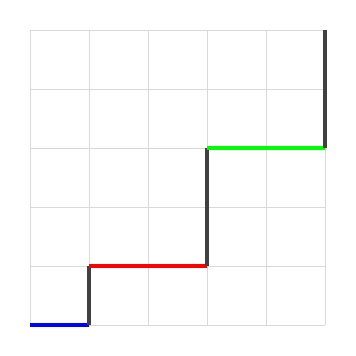
\begin{tikzpicture}[scale=0.75]
    \draw[help lines, color=gray!30] (0,0) grid (5,5);
    
    \draw[ultra thick, blue] (0,0) -| (1,0);
    \draw[ultra thick, darkgray] (1,0) -| (1,1);
    \draw[ultra thick, red] (1,1) -| (3,1);
    \draw[ultra thick, darkgray] (3,1) -| (3,3);
    \draw[ultra thick, green] (3,3) -| (5,3);
    \draw[ultra thick, darkgray] (5,3) -| (5,5);
    \end{tikzpicture}
    \end{center}
    \end{enumerate}
\end{frame}

%%%%%%%%%%%%%%%%%%%%%%%


\begin{frame}{What is $\mathcal{D}_n$?}

    \begin{block}{Definition}
    \textbf{Dyck path:} A lattice path in the plane $\mathbb{Z}^2$ consisting of UP (diagonally) $\nearrow$ steps $(1,1)$ and DOWN (diagonally) $\searrow$  steps  $(1,-1)$ which goes from $(0,0)$ to $(2n,0)$ and never goes below the $x$-axis.

    Let $\mathcal{D}_n$ be the set of Dyck paths from $(0, 0)$ to $(2n, 0)$.

    We have: $|\mathcal{D}_n| = C_n$.
    \end{block}
    \begin{figure}
        \centering
        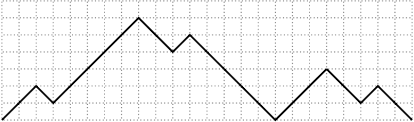
\includegraphics[width=0.5\linewidth]{media/dyck_path.png}
        \caption{Dyck path}
        \label{fig:dyck-path-example}
    \end{figure}
\end{frame}

\begin{frame}{Bijection between $\mathcal{S}_n(132)$ and $\mathcal{D}_n$}

    There exists a \textbf{bijection} between $\mathcal{S}_n(132)$ and $\mathcal{D}_n$ or we can map each $\pi \in \mathcal{S}_n(132)$ to a corresponding Dyck path from $(0,0)$ to $(2n,0)$.
    
    With each element $\pi_i$ of $\pi \in \mathcal{S}_n(132)$ ($1 \leq i \leq n$), we can draw a Dyck path going from $(0,0)$ to $(2n,0)$ following these steps:

\begin{enumerate}
    \item We define $h_i$, the number of elements in $\pi_{i+1}\pi_{i+2}\ldots \pi_{n}$ that are larger than $\pi_i$
    \item We go $\nearrow$ for a sufficient number of steps (or we can stay at the same position) such that we arrive at the point $(x,y)$ that has $y=h_i + 1$ 
    \item We go $\searrow$ for one step from $(x,y)$ to $(x + 1,y - 1)$
\end{enumerate}

\end{frame}

\begin{frame}{Bijection between $\mathcal{S}_n(132)$ and $\mathcal{D}_n$}

    \begin{figure}[htbp]
        \centering
       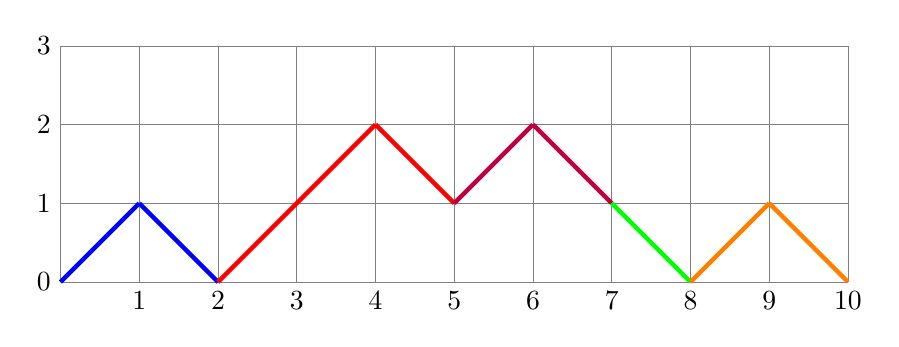
\begin{tikzpicture}[scale=1][H]
        % Draw the grid and diagonal
        \draw[help lines] (0,0) grid (10,3);
    
        \node[left] at (0,0) {0};
        \node[left] at (0,1) {1};
        \node[left] at (0,2) {2};
        \node[left] at (0,3) {3};
        \node[below] at (1,0) {1};
        \node[below] at (2,0) {2};
        \node[below] at (3,0) {3};
        \node[below] at (4,0) {4};
        \node[below] at (5,0) {5};
        \node[below] at (6,0) {6};
        \node[below] at (7,0) {7};
        \node[below] at (8,0) {8};
        \node[below] at (9,0) {9};
        \node[below] at (10,0) {10};
        \draw[ultra thick, blue] (0,0) -- (1,1);
        \draw[ultra thick, blue] (1,1) -- (2,0);
        \draw[ultra thick, red] (2,0) -- (4,2);
        \draw[ultra thick, red] (4,2) -- (5,1);
        \draw[ultra thick, purple] (5,1) -- (6,2);
        \draw[ultra thick, purple] (6,2) -- (7,1);
        \draw[ultra thick,  green] (7,1) -- (8,0);
        \draw[ultra thick,  orange] (8,0) -- (9,1);
        \draw[ultra thick, orange] (9,1) -- (10,0);
    \end{tikzpicture}
    \caption{Dyck path mapped from $\pi=5\;3\;2\;4\;1$}
    \end{figure}
\end{frame}

\begin{frame}{Bijection between $\mathcal{S}_n(132)$ and $\mathcal{D}_n$}
    \begin{figure}[htbp]
    \centering
    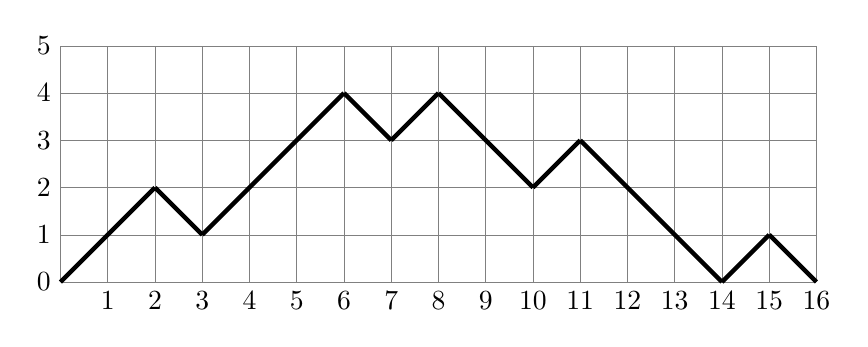
\begin{tikzpicture}[scale=0.6][H]
        % Draw the grid and diagonal
        \draw[help lines] (0,0) grid (16,5);
    
        \node[left] at (0,0) {0};
        \node[left] at (0,1) {1};
        \node[left] at (0,2) {2};
        \node[left] at (0,3) {3};
        \node[left] at (0,4) {4};
        \node[left] at (0,5) {5};
        \node[below] at (1,0) {1};
        \node[below] at (2,0) {2};
        \node[below] at (3,0) {3};
        \node[below] at (4,0) {4};
        \node[below] at (5,0) {5};
        \node[below] at (6,0) {6};
        \node[below] at (7,0) {7};
        \node[below] at (8,0) {8};
        \node[below] at (9,0) {9};
        \node[below] at (10,0) {10};
        \node[below] at (11,0) {11};
        \node[below] at (12,0) {12};
        \node[below] at (13,0) {13};
        \node[below] at (14,0) {14};
        \node[below] at (15,0) {15};
        \node[below] at (16,0) {16};
        \draw[ultra thick,  black] (0,0) -- (2,2);
        \draw[ultra thick,  black] (2,2) -- (3,1);
        \draw[ultra thick, black] (3,1) -- (6,4);
        \draw[ultra thick, black] (6,4) -- (7,3);
        \draw[ultra thick, black] (7,3) -- (8,4);
        \draw[ultra thick, black] (8,4) -- (10,2);
        \draw[ultra thick, black] (10,2) -- (11,3);
        \draw[ultra thick, black] (11,3) -- (14,0);
        \draw[ultra thick, black] (14,0) -- (15,1);
        \draw[ultra thick, black] (15,1) -- (16,0);
    \end{tikzpicture}
    \caption{Dyck path mapped from $\pi=7\;4\;3\;5\;2\;6\;8\;1$}
    \end{figure}
\end{frame}

\begin{frame}{Bijection between $\mathcal{S}_n(132)$ and $\mathcal{D}_n$}
    We can conclude that $s_n(132) = Cn$. Since $\{132,213,231,312\}$ is the set of Wilf equivalent patterns, we can confidently conclude that $s_n(132) = s_n(213) = s_n(132) = s_n(312)=C_n$.

    From above, we know that $s_n(321)=s_n(123)=C_n$ (Wilf equivalent). Therefore, we have:
    $$s_n(132) = s_n(213) = s_n(132) = s_n(312)=s_n(321)=s_n(123)$$

    \begin{block}{Proposition}
    All of the patterns of length $3$ are Wilf equivalent, and $s_n(\sigma)$ with $\sigma$ of length $3$ is equal to $C_n$.
    \end{block}
\end{frame}
%%%%%%%%%%%%%%%%%%%%%%%
\begin{frame}{Bijection between $\mathcal{S}_n(123)$ and $\mathcal{D}_n$}
    \begin{block}{Definition}
    \textbf{Right-to-Left Maximum:} An element of a permutation that is larger than every element to its right.
    \\
    Example: 4\;1\;2\;6\;3\;\underline7\;\underline5
    \end{block}
    
    Iterating over a permutation $\pi \in \mathcal{S}_n(123)$ from right to left, we find the right-to-left maximum. Let $M_{n}$ be the set of the right-to-left maxima collected when we iterate over $\pi$ from right to left, and $s = |M_n|$. We denote the consecutive subsequence of $\pi$ between $m_{i+1}$ and $m_i$ as $w_i$.
    
    $$\pi = w_sm_sw_{s-1}m_{s-1}\ldots w_1s_1$$

    \end{frame}

\begin{frame}{Bijection between $\mathcal{S}_n(123)$ and $\mathcal{D}_n$}
    For $1 \leq i \leq s$, we follow the steps below to create a Dyck path:
\begin{enumerate}
     \item We take $m_i - m_{i+1}$ $\nearrow$ steps.
     \item For every consecutive subsequence $w_i$, we take $|w_i| + 1$ $\searrow$ steps ($|w_i|$ is the number of elements of $w_i$).
 \end{enumerate}

\begin{figure}
    \centering
    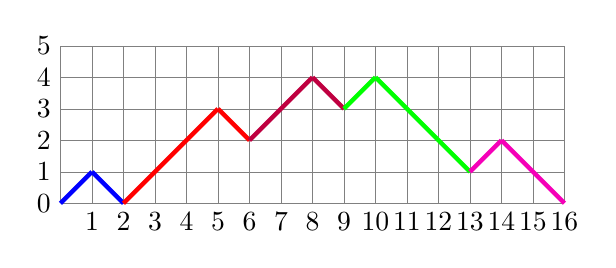
\begin{tikzpicture}[scale=.4][H]
    \draw[help lines] (0,0) grid (16,5);

    \node[left] at (0,0) {0};
    \node[left] at (0,1) {1};
    \node[left] at (0,2) {2};
    \node[left] at (0,3) {3};
    \node[left] at (0,4) {4};
    \node[left] at (0,5) {5};
    \node[below] at (1,0) {1};
    \node[below] at (2,0) {2};
    \node[below] at (3,0) {3};
    \node[below] at (4,0) {4};
    \node[below] at (5,0) {5};
    \node[below] at (6,0) {6};
    \node[below] at (7,0) {7};
    \node[below] at (8,0) {8};
    \node[below] at (9,0) {9};
    \node[below] at (10,0) {10};
    \node[below] at (11,0) {11};
    \node[below] at (12,0) {12};
    \node[below] at (13,0) {13};
    \node[below] at (14,0) {14};
    \node[below] at (15,0) {15};
    \node[below] at (16,0) {16};
    \draw[ultra thick, blue] (0,0) -- (1,1);
    \draw[ultra thick, blue] (1,1) -- (2,0);
    \draw[ultra thick, red] (2,0) -- (5,3);
    \draw[ultra thick, red] (5,3) -- (6,2);
    \draw[ultra thick, purple] (6,2) -- (8,4);
    \draw[ultra thick, purple] (8,4) -- (9,3);
    \draw[ultra thick, green] (9,3) -- (10,4);
    \draw[ultra thick, green] (10,4) -- (13,1);
    \draw[ultra thick,  magenta] (13,1) -- (14,2);
    \draw[ultra thick,  magenta] (14,2) -- (16,0);
\end{tikzpicture}
\caption{Dyck path created from $\pi=5\;8\;3\;2\;7\;6\;4\;1$ following the steps above}
\end{figure}
\textcolor{red}{HOWEVER, IT'S NOT DONE YET!!!!}
\end{frame}

\begin{frame}{Bijection between $\mathcal{S}_n(123)$ and $\mathcal{D}_n$}

We need to reflect the newly generated Dyck path over a vertical line. Finally, we get the corresponding Dyck path.

\begin{figure}
    \centering
    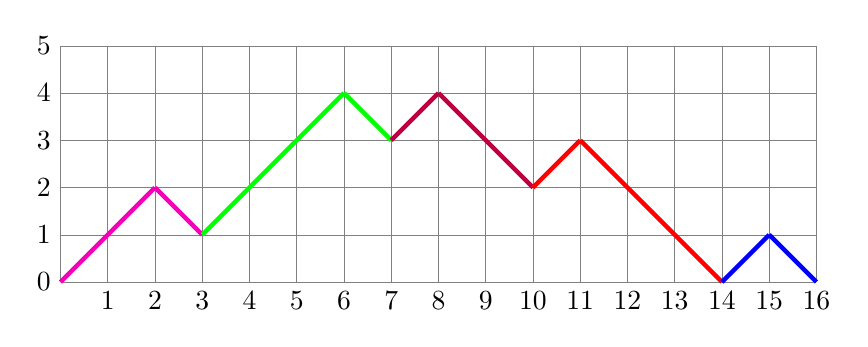
\begin{tikzpicture}[scale=0.6][H]
    \draw[help lines] (0,0) grid (16,5);

    \node[left] at (0,0) {0};
    \node[left] at (0,1) {1};
    \node[left] at (0,2) {2};
    \node[left] at (0,3) {3};
    \node[left] at (0,4) {4};
    \node[left] at (0,5) {5};
    \node[below] at (1,0) {1};
    \node[below] at (2,0) {2};
    \node[below] at (3,0) {3};
    \node[below] at (4,0) {4};
    \node[below] at (5,0) {5};
    \node[below] at (6,0) {6};
    \node[below] at (7,0) {7};
    \node[below] at (8,0) {8};
    \node[below] at (9,0) {9};
    \node[below] at (10,0) {10};
    \node[below] at (11,0) {11};
    \node[below] at (12,0) {12};
    \node[below] at (13,0) {13};
    \node[below] at (14,0) {14};
    \node[below] at (15,0) {15};
    \node[below] at (16,0) {16};
    \draw[ultra thick,  magenta] (0,0) -- (2,2);
    \draw[ultra thick,  magenta] (2,2) -- (3,1);
    \draw[ultra thick, green] (3,1) -- (6,4);
    \draw[ultra thick, green] (6,4) -- (7,3);
    \draw[ultra thick, purple] (7,3) -- (8,4);
    \draw[ultra thick, purple] (8,4) -- (10,2);
    \draw[ultra thick, red] (10,2) -- (11,3);
    \draw[ultra thick, red] (11,3) -- (14,0);
    \draw[ultra thick, blue] (14,0) -- (15,1);
    \draw[ultra thick, blue] (15,1) -- (16,0);
\end{tikzpicture}
    \caption{Dyck path mapped from $\pi=5\;8\;3\;2\;7\;6\;4\;1$ (it looks familar, right?)}
\end{figure}
\end{frame}

%%%%%%%%%%%%%%%%%%%%%%%

\begin{frame}
\frametitle{Classical Pattern Avoidance}
\begin{block}{Patterns of length 4}
    $S_4 = \{1234,1342,1324\}$
\end{block}

Formulas:

$s_n(1234) = \frac{1}{(n+1)^2(n+2)}\sum\limits_{k=0}^n\binom{2k}{k}\binom{n+1}{k+1}\binom{n+2}{k+1}$

$s_n(1342) = (-1)^{n-1}\left(\frac{7n^2-3n-2}{2}\right)+3\sum\limits_{i=0}^n(-1)^{n-i}2^{i+1}\frac{(2i-4)!}{i!(i-2)!}\binom{n-i+2}{2}$

\begin{center}
current area of study $ \longrightarrow{\bf s_n(1324) = ???}$ 
\end{center}

"Zeilberger has said “Not even God knows the number of 1324-avoiders of length 1000”. While making no Messianic claims, our asymptotics permit the approximate answer $5 + 1 \times 10^{1017}$"
\begin{flushright}
- Conway and  Guttmann, 2015
\end{flushright}
\end{frame}


\begin{frame}
\frametitle{Generalized Pattern Avoidance} 
\begin{block}{Definition}
A {\bf generalized pattern} is a permutation in which a dash may or may not exist between each digit. Some permutation $\pi$ is said to contain this pattern if there exists some subsequence in $\pi$ where the pattern occurs and there are no digits separating the adjacent parts of the pattern.
\end{block}

Ex: $615243$

\hspace{1cm} \underline{Contains} (41-23)$ \rightarrow\    \textcolor{red}{61}5\textcolor{red}{24}3$

\hspace{1cm} \underline{Avoids} (4-123)$ \rightarrow\ 
 61\textcolor{red}{5}243$

\vspace{2cm}

\end{frame}

\begin{frame}
\frametitle{Generalized Pattern Avoidance}

{\bf Generalized patterns increase the number of connections to other concepts and sequences}
\vskip11pt
\begin{prop}
    The number of 1-32 avoiding permutations of length $n$, $s_n(1-32)$, is equivalent to the number of ways the sequence $\{123...n\}$ can be divided into non-empty sets.
\end{prop}

ex: $\{\{23\},\{1\}\} \rightarrow$ avoids $(1-32)$

\vskip11pt
**Bijection comes from standardizing how the divided sequence is written
\end{frame}

\begin{frame}{Pattern Strongly Avoiding Permutation}

\begin{exampleblock}{Example of square of permutation $\pi^2$}
    We have $\pi = 1\;3\;4\;2 \in [4]$. 
    
     $$1\;2\;3\;4 \rightarrow 1\;3\;4\;2  \rightarrow 1\;4\;2\;3$$
\end{exampleblock}
\begin{block}{Definition}
    Let $\sigma$ be a permutation of the set $[m]$ where $m \leq n$ such that $\pi$ avoids $\sigma$. We can say that $\pi$ is strongly $\sigma-$avoiding\index{strongly $\sigma-$avoiding} if both $\pi$ and $\pi^2$ avoid $\sigma$.

    The number of strongly $\sigma$-avoiding permutations of $[n]$ is $Sav_n(\sigma)$.
\end{block}

\textcolor{red}{Special case:} If $\sigma = 1\;2\;3\ldots\;m$ (a strictly increasing pattern) and $n \geq (m-1)^3 + 1$, we have: 
$$Sav_n(\sigma)=0$$


\end{frame}

\begin{frame}{Pattern Strongly Avoiding Permutation}
Two symmetric equivalences:

\begin{prop} Let $\sigma$ be a pattern, and $\sigma^{-1}$ be the inverse of $\sigma$. Then we have:

$$Sav_n(\sigma)=Sav_n(\sigma^{-1})$$
\end{prop}

\begin{prop} Let $\sigma$ be a pattern of length $m$, and $\sigma^{'}$ be the reverse complement of $\sigma$ (we reverse the order of $\sigma$, then replace each element $\sigma_i$ with $m+1-\sigma_i$). Then we have:

$$Sav_n(\sigma)=Sav_n(\sigma^{'})$$
\end{prop}

\end{frame}

\begin{frame}
    \begin{center}
        \Huge \textbf{Application: Stack Sorting Algorithms}
    \end{center}
\end{frame}

\begin{frame}{Pattern Strongly Avoiding Permutation}
    \frametitle{Sorting With Stacks}
    \begin{enumerate}
        \item Sorting
        \item Permutations and data structures
        \item Stacks are first-in-first-out with two operations
        \item A bit like a hole in the ground...
        \item Condition for result to be sorted
    \end{enumerate} 
    \begin{center}
        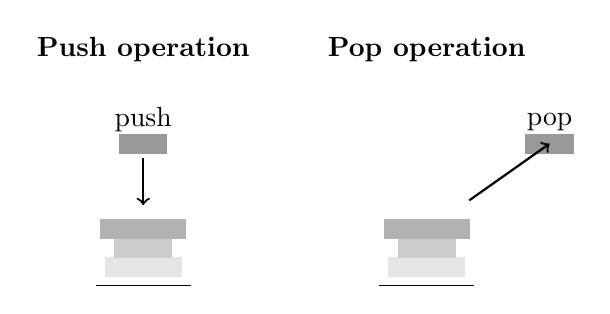
\begin{tikzpicture}[scale=.6]
        
        % left
        \node at (0,5) {\textbf{Push operation}};
        
        % stack base
        \draw (-1,0) -- (1,0);
        
        % plates (bottom to top, top one moved above arrow)
        \filldraw[gray!20] (-0.8,0.2) rectangle (0.8,0.6);
        \filldraw[gray!40] (-0.6,0.6) rectangle (0.6,1.0);
        \filldraw[gray!60] (-0.9,1.0) rectangle (0.9,1.4);
        
        % arrow showing push
        \draw[->, thick] (0,2.7) -- (0,1.7);
        \node at (0,3.5) {push};
        
        \filldraw[gray!80] (-0.5,2.8) rectangle (0.5,3.2);
        
        
        % right
        \node at (6,5) {\textbf{Pop operation}};
        
        % stack base
        \draw (5,0) -- (7,0);
        
        % plates
        \filldraw[gray!20] (5.2,0.2) rectangle (6.8,0.6);
        \filldraw[gray!40] (5.4,0.6) rectangle (6.6,1.0);
        \filldraw[gray!60] (5.1,1.0) rectangle (6.9,1.4);
        
        % arrow showing pop
        
        \filldraw[gray!80] (8.1,2.8) rectangle (9.1,3.2);
        
        \node at (8.6,3.45) {pop};
        
        \draw[->, thick] (6.9,1.8) -- (8.6,3);
        
        \end{tikzpicture}
        \end{center}
    \begin{center}
        
    \end{center}
\end{frame}

\begin{frame}{Pattern Strongly Avoiding Permutation}
    \frametitle{Sorting With Stacks}
    \begin{center}
    \scalebox{0.6}{
    \begin{algorithm}[H]
    \DontPrintSemicolon
        \KwIn{A list $P$ of $n$ items with ordered form $\{a_1,a_2,\ldots,a_n\}$}
        \KwOut{A new list $P'$}
        $S\leftarrow$ An empty stack\\
        \While{The size of $P'$ is less than $n$}{
            \If{$P$ is empty}{
                Pop $a_i$ from $S$ and append it to $P'$
            }
            \ElseIf{$S$ is empty}{
                Push the first element of $P$ onto $S$ and remove it from $P$
            }
            \ElseIf{The top of $S$ is greater than $P$[0]}{
                Push the first element of $P$ onto $S$ and remove it from $P$
            }
            \Else{
                Pop $a_i$ from $S$ and append it to $P'$
            }
        }
        \caption{Stack Sorting With One Stack (\texttt{stack\_sort})}
    \end{algorithm}
    }
    \end{center}
\end{frame}

\begin{frame}{Pattern Strongly Avoiding Permutation}
    \frametitle{Sorting With Stacks}
    \begin{prop}
        Let $P$ be a permutation of $\{1,2,\ldots,n\}$ where $n$ is in position $i$, so that $P=k_1k_2\ldots k_{i-1}nk_{i+1}\ldots k_n$. Then \begin{center}\texttt{stacksort}$(P)=$\texttt{stacksort}$(k_1\ldots k_{i-1})$\texttt{stacksort}$(k_{i+1}\ldots k_n)n$.
        \end{center}
    \end{prop}
    The recursive definition helps us see how $n$ form length-three patterns with elements to its left and right, relating the problem to avoiding the pattern 231. \\
    One may also choose to think about the algorithm as a string of Xs and Ys, where X represents push and Y is pop. This gets us closer to solving the more general question of stack-sortable permutations. In the end, the greedy algorithm is representative of every stack-sortable permutation.
\end{frame}

\begin{frame}{Pattern Strongly Avoiding Permutation}
    \frametitle{Sorting With Deques}
    \begin{enumerate}
        \item What is a double-ended queue (deque)?
        \item Input (IRD) and output (ORD) restricted deques
        \item Main question: how many permutations can be sorted by IRDs?
    \end{enumerate}

    For a string of X, Y, and Z:
    \begin{enumerate}
        \item According to an IRD, Z pushes to top, X pops bottom, and Y pops top
        \item According to an ORD, Z pops bottom, X pushes to top, and Y pushes to bottom
    \end{enumerate}
    
\end{frame}

\begin{frame}{Sorting With Deques}
Let's reframe the problem with bijection:
    \begin{defn}
        A string is admissible when it satisfies the following conditions:
        \begin{enumerate}
            \item There are $n$ Zs and $n$ combined Xs and Ys.
            \item Reading from left to right, Zs never exceed the combined Xs and Ys.
            \item Whenever Zs equal Xs and Ys, if there are not yet $2n$ characters, the next character is an X.
            \item The substring XZ does not occur.
        \end{enumerate}
    \end{defn}
    \begin{enumerate}
        \item Rules 1 and 2 are obvious
        \item Rules 3 and 4 prevent redundancy
    \end{enumerate}

    
\end{frame}

\begin{frame}{Sorting With Deques}
    Reframing the problem:
    \begin{prop}
        The number of IRD-sortable permutations of size $n$ is equal to the number of permutations of $n$ elements that can be obtained from passing a permutation through an ORD.
    \end{prop}
    \begin{enumerate}
        \item Each sortable permutation $\sigma$ of $n$ elements has a unique admissible string that sorts it by IRD
        \item An ORD reading that admissible string in reverse generates $\sigma$ from the sorted permutation
    \end{enumerate}
\end{frame}

\begin{frame}{Producing Permutations With Deques}
    Consider the number of strings with $n$ total symbols and $m$ more pushes than pops that are otherwise admissible. Denote all such strings which end in Z with the sequence $\{h_{n,m}\}$ and all those that do not with $\{g_{n,m}\}$. Our two recurrences are $$g_{n+1,m}=2g_{n,m-1}+h_{n,m-1}$$ $$h_{n+1,m}=g_{n,m+1}+h_{n,m+1}.$$
\end{frame}

\begin{frame}{Producing Permutations With Deques}
    Bivariate generating functions:
    $$G(x,y)=\sum\limits_{n,m=0}^\infty g_{n,m}x^my^n,\ H(x,y)=\sum\limits_{n,m=0}^\infty h_{n,m}x^my^n.$$
    Standard combinatorial recursive nonsense gives:
    $$\frac{G(x,y)}{y}=2xG(x,y)+x\left(H(x,y)-h(y)\right)+x$$
    $$\frac{H(x,y)}{y}=\frac{G(x,y)}{x}+\frac{H(x,y)-h(y)}{x}$$

    We want to find $h(y)$, which represents $h_{n,0}$.
\end{frame}

\begin{frame}{Kernel Method}
    Using substitution, solving for $G$, and doing some algebra, we arrive at this function.
    $$G(x,y)==\frac{xy(x-y-xh(y))}{-2yx^2+(1-y^2)x-y}$$
    Factoring the quadratic denominator gives
    $$r_1(y),r_2(y)=\frac{-(1+y^2)\pm\sqrt{(1+y^2)^2-4(-2y)(-y)}}{-4y}.$$
    So the denominator is zero when $x=r_1(y)$; the kernel method is determining $h(y)$ by setting the numerator equal to zero as well.
\end{frame}

\begin{frame}{Schröder Numbers}
    Our final generating function is 
    $$h(y)=\frac{3-y-\sqrt{1-6y+y^2}}{2}$$
    which looks like 
    $$1+y+2 y^2+6 y^3+22 y^4+90 y^5+394 y^6+1806 y^7+8558 y^8+41586 y^9+\ldots$$
    These are the Schröder numbers! They count 4231 and 3241 avoiding permutations.
\end{frame}

\begin{frame}{Results}
    \begin{figure}[htbp]
    \centering
    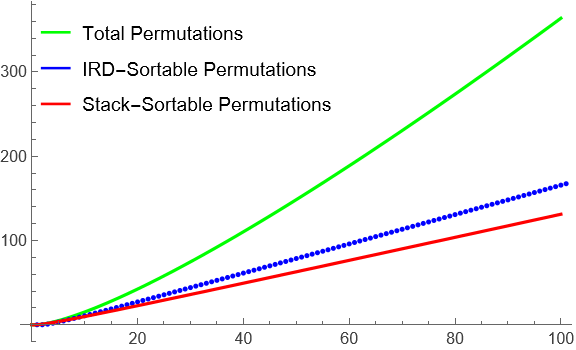
\includegraphics[width=.7\textwidth]{media/sort_plot.png}
    \caption{On the x-axis we have $n$, and, on the y-axis, we have the number of different groups of permutations on a log scale.}
    \label{fig:example}    
\end{figure}
\end{frame}

\begin{frame}{Stack Systems}
     In theory, $\log_2n$ stacks in sequence can sort any permutation. In practice? Well...
\end{frame}

\begin{frame}
    \begin{center}
        \Huge \textbf{Thank You for Listening to Our Presentation!}
    \end{center}
\end{frame}

\end{document}